\chapter[Future Work]{Future Work} \label{appendix-future-work}

% TODO PUT THIS INTO THE BODY OF THE TEXT BEFORE CONCLUSION?

% In  this chapter, we discuss potential extensions of our basic model. 
Our goal has been to make a simple model that illustrates essential principles like the % model as simple as the 
Alonzo model \cite{alonsoLocationLandUse1964}. We have sharply restricted our model  in order to focus on one process of significance, financialization.  %This is in part so that we can explain and justify each assumption that we use, and in part because building from sharply restricted helps to create understandable results.  
% Those results are condition on the specific set of assumptions to ensure that 
We have nevertheless designed the model to accommodate a range of extensions to explore questions that are theoretically or interesting or important for policy-makers. 
In this chapter, we explain the choices for what is included and excluded from the model and then describe potential extensions.

There are several illustrative classes of extension. Figure~\ref{fig-extensions-logic} illustrates five general types of extension to the base model.  In each case, we introduce the class and give several examples. 

The first is to move from a static population to a model with population pressure. % This appears on the left as a group of three new subroutines with connections to the elements of the model most directly affected. % Some links are left out to keep the figure readable. Examples of omitted links  are the channels through which  population affects labour supply and savings.  
A second class of extension would introduce a housing production sector. This appears on the right side of of the figure linked to the banking sector. It requires adding a dynamic housing stock. 
A third class of extensions, separable from production is to introduce variation of housing form,  density and amenity. Zoning restrictions and building codes are related. Many questions about who gets what housing arise at this point. 

{\newpage\thispagestyle{empty}
\vspace{-1.5cm}
\begin{figure}
\vspace{-4.5cm}
\begin{adjustwidth}{-0.24\textwidth}{-0.2\textwidth}
\centering
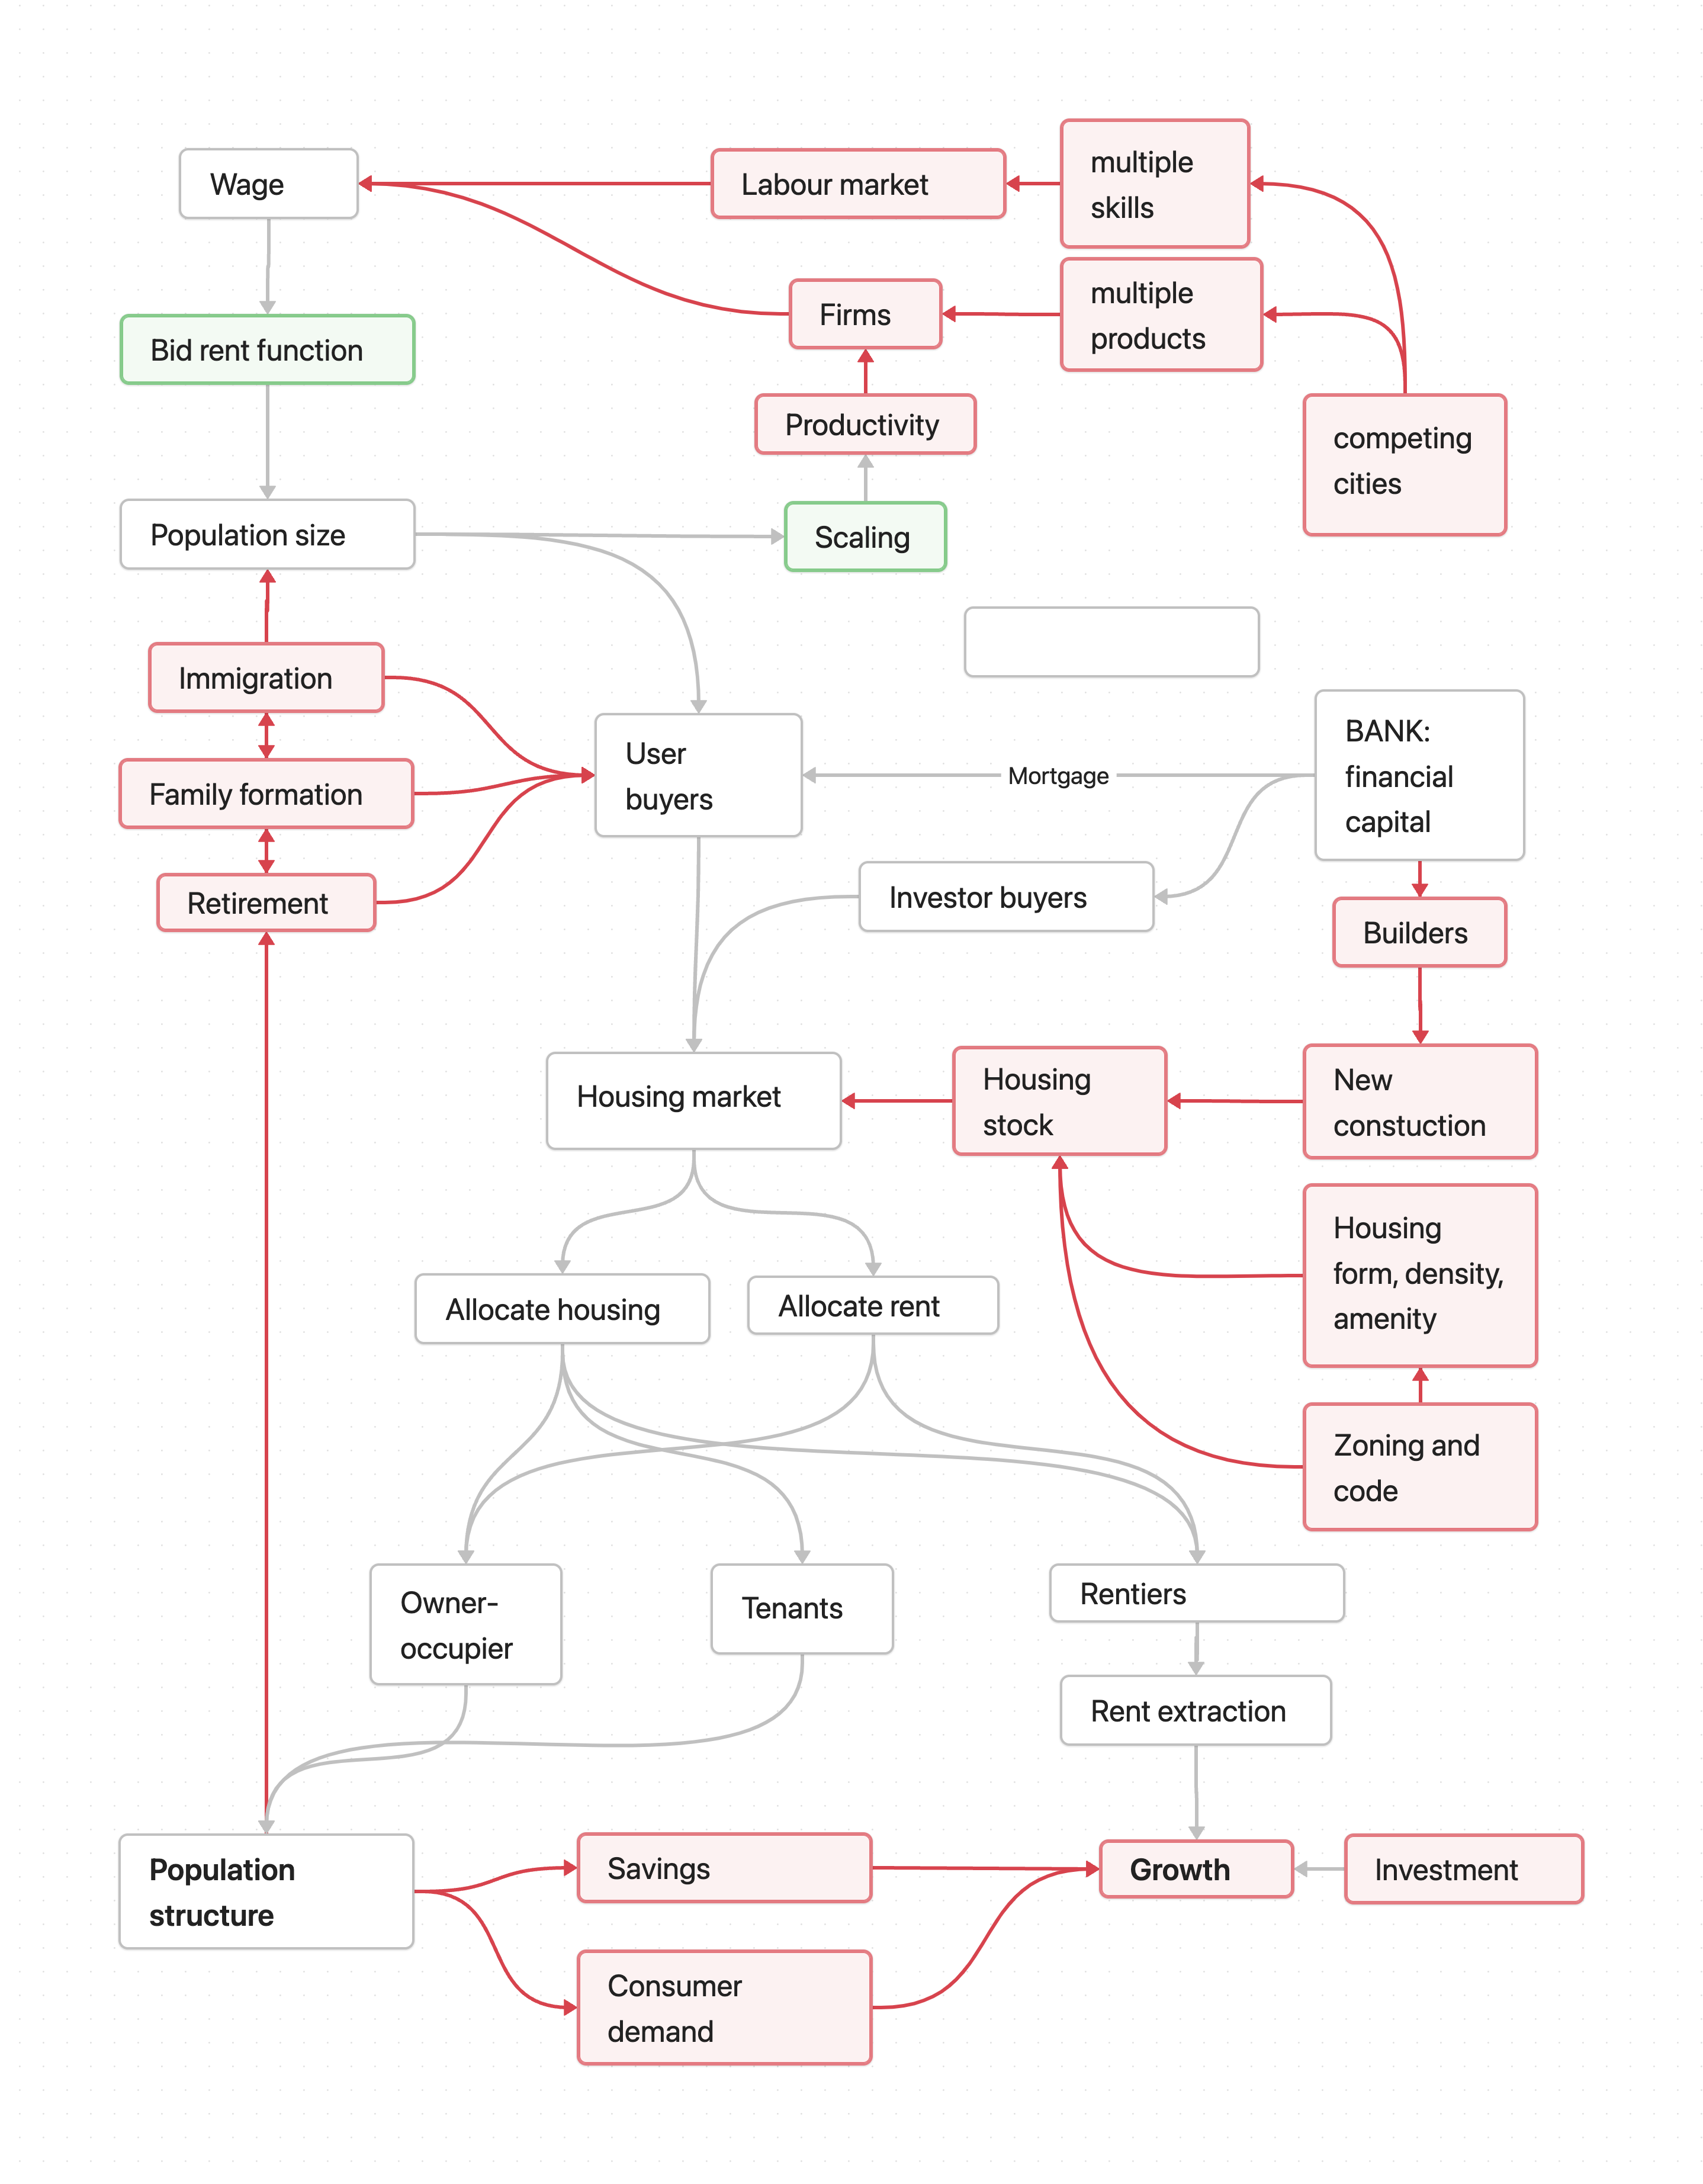
\includegraphics[scale=.22]{fig/extensions-logic.png}
\end{adjustwidth}
\caption{Extensions}
\label{fig-extensions-logic}
%\pagestyle{headings}
% \usetikzlibrary{positioning}
%\begin{tikzpicture}[remember picture,overlay,shift={(current page.north east)}] \node[anchor=north east,xshift=-1cm,yshift=-1cm]{\includegraphics[width=1cm]{example-image-a}};\end{tikzpicture}
\end{figure}}

At the bottom of the figure we introduce a fourth class of intervention, consumer demand linked to the population structure and feeding back to growth. Savings behaviour becomes more  complex when consumer demand is made endogenous and with as more complex population structure.

The fifth block of extensions illustrated in Figure~\ref{fig-extensions-logic} would replace the simple, scaling-based transmission mechanism in the Alonso-Jacobs cycle with explicit firm and labour market behaviour. This class of extensions is obviously linked to population structure. It leads to consideration of firms that produce different products, some for export some for the local market, and to multiple types of labour.
Linked to the labour market and production system is the possibility of introducing competing cities. 

% It should be clear that e

%We would argue that none of them would change our qualitative results greatly, although each would deepen our understanding of mechanisms and of the detailed impacts.

There are many more possible models than this, and these extensions combine. Models are by nature combinatoric: every added element involves making a choice among alternative assumptions and implementations. Each extension is potentially as complex as the core model, and each introduces additional assumptions.  A model incorporating in binary choices is one of an implicit family of $2^n$ alternative models. 
They also describe a particular logic, which may be explored or studied in any particular region or context, drawing on local data and estimated parameter values. The context will also suggest, in many cases theoretical extensions, or particular questions.

\section{Population pressure} 
Our basic model does not have a growing population. This conveniently allows us to isolate certain effects of financialization. Population pressure is one of the drivers of financialization because it amplifies speculative gains, however. As a result, one of the first extensions must be  to introduce population pressure.

There are two sources to consider: 
\begin{enumerate}
\item agglomeration effects that increase the wage and attract workers faster than the housing stock can respond. 

Worker agents from outside the city can always consider moving and accepting a job. 
% QUESTION - how to manage the flow of new agents?
%, or can make more from rents and moving away
\item immigration pressure.
\end{enumerate}
Under the  first, agglomeration economies drive population while under the second, population growth may drive agglomeration.

The growth of the housing stock will generally lag population growth, generating price effects and stock dynamics.
Agents will respond to increases in demand conditions. The perception that the market is tight or that prices are rising may lead to higher bids and reservation prices and shift results in favour of sellers.  


%Buyers could consider neighbourhood pressures, demographic changes, changes in job location, desire for amenity etc. in their assessment of housing need. 

%With multiple bids agents can place the most competitive bids on those homes they prefer. If they have higher urgency they place strong bids on more homes. 

%Next buyers request a selection of homes to consider from a real estate agent. Those with higher need for housing look at more homes. The real estate agent offers a selection of homes based on the agent's requirements. A randomness parameter determines how many divergent houses are also considered. When the parameter is 1, the selection of homes is fully randomized, When it is 0, the agent sorts all available homes and offers those which fit the agents budget, space, and other requirements best.

\section{Retirement, investors, and private investment properties}
The simple population turnover in our model can be replaced with a more complex set of possibilities at the agent level.  At retirement,  agents can be allowed to may choose between selling their home, renting it as an income property, or if there is sufficient amenity value for them, staying in the city. Implementing these choices complicates the agent decision and the resulting housing distribution but require few changes to the rest of the model.

\section{Housing production}

\section{Differences in density, housing form, and neighbourhood amenity}
Much of what is interesting in a city is the rich variety of housing forms and neighbourhoods and the varied populations that occupy them. Our model has a single form of housing and an undifferentiated populations, allowing us to differentiate the housing system in specific ways and study the interactions between the built world and the population. We are convinced that few of the possible extensions could affect our qualitative results. 

Nonetheless, in our agent based model, in which every lot is  addressable, it is simple to introduce zoning boundaries, local amenities, different densities or housing qualities and homes of different sizes. Hundreds of experiments are possible exploiting  the extensibility we have carefully conserved.  

We can ask what would be the effect of a hard zoning boundary and what would be the effect of suddenly relaxing it. We could explore the effect of speeding the rate of conversions from one size  home to another, or of locating high density pocket on a transportation route. Many significant urban policy questions could be examined with a limited amount of additional programming. 

\section{The consumer city}
Much of the demand for what is produced in the city is local consumer demand.  Our model has assumed there is production only for a perfectly elastic export demand. Consumer needs are buried in the subsistence wage. 

A minimal extension would be to introduce a second sector representing local consumption demand. A share of locally generated income would support production for the city's population. The labour force would be split between the two sectors and both productivity and wages might differ across sectors. 
A more complex treatment would introduce a range of service, entertainment and retail producers. This might be done monopolistically competitive firms \'a la Dixit and Stiglitz \cite{AvinashK.Dixit1977MCaO}.



\section{Distribution of rents}
Rents go to landowners, with a share taken for maintenance and taxes.
Rents may also be taxed, could be shared between multiple owners, etc.
 %\note{REPHRASE? rent is  extracted from the coalition of capital and workers.} % Rents may also be taxed, could be shared between multiple owners, etc. 
%The rents are captured by landowners.  The capture of rents by landowners is common buy not necessary. 
In principle the gains from urban productivity and amenity can be allocated as social wealth through shared ownership, as is often done on a small scale with cooperatives and land trusts, distributed to all citizens through something like a social wealth fund, or captured in taxes or fees as Henry George suggested. 
%The rents would otherwise go to labour and capital.





\section{Urban savings}
% TODO THIS IS A CONTRIBUTION, BUT ALSO A DISCUSSION OF ONE WAY THIS WORK COULD BE EXTENDED, MIXED WITH A BIT OF MODEL DESCRIPTION

Conventional growth models specify a savings/investment mechanism at the national level. To our knowledge, this has not been done for the city level. We require  savings at two levels. First, since we want to incorporate  households home ownership and a relationship to the financial sector through mortgages, We specify a savings rate out of the spending we have isolated in the `subsistence wage' This means that both urban and rural workers accumulate savings, that savings are age-dependent, making the size of mortgage available also age dependent. 

Homeowners in addition have equity $E=P-M$ in their homes. % ({\color{red}Should newcomers also have equity? or is it built into the savings. Clarify this.} 

A second level of saving is the  investment in capital out of the city surplus. Even raising this question puts us into terra incognita. There are many  channels through which surplus flows into productive investment in the urban contest. One is through public investment in infrastructure. We have discussed how falling transportation costs increase surplus generation. Investments like this are made slowly and take effect over time periods much longer than our model is concerned with.  We can set a property tax rate   that we will assume is sufficient to maintain the stock of infrastructure.

Public and private investment in human capital is largely urban as well, but as with infrastructure, investment and response take effect over time periods much longer than our model is concerned with. 

Private sector innovation in technology, marketing, or products draws on local saving less but still significantly on local savings. We have little in the way of theory or empirical research on this channel. Lags between investment and any rise in the urban wage premium are almost certainly long and variable. 

We deal with this issue by linking local capital ownership with the scale factor. It is known that local ownership is associated with local investment. We will assume that local capital ownership, which consists in part of local ownership of the housing stock, can be proxied by homeowner equity as a share of local. 

\section{Savings and retirement behaviour}
Agents fund their retirement from savings, as well as returns on their home if they have one to sell. Savings may be invested in a pension fund, or in local property,  depending on expected risks and returns. In the real world, financial institution manages most pensions, investing in the market or in property.  All this institutional structure is probably most easily handled by implementing a savings account for each agent. We are not interested in the detailed investment behavour for the financial sector.% either in the stock market, or in pensions.

%Institutional and individual investors can access debt. %

We could also consider a case where outside money can come under institutional management, not just local retirement savings. A parameter would control the inflow of additional money beyond local investment in the pension fund. 

\section{Making labour market and firm behaviour explicit}
We have carefully developed the link between neoclassical growth theory and the literature on urban scaling \cite{bettencourtIntroductionUrbanScience2021} and  We then imposed the scaling result on our model.  We force the model to conform to the empirical data on the relationship between population and productivity. This amounts to black-boxing the entire production and labour demand sector as well as the construction and housing production sector. 

This made sense because our focus  was on the housing market and the financial sector, but the model we have constructed will allow us to ``fill the black box'' with more complete models of the production and labour market to see how they compare to the empirical data. 

The  scaling  literature also provides relationships between density and population and infrastructure cost and population that we can explore in the same way. In the scaling literature, these relationships are increasingly theorized in terms of network effects, which is perfectly consistent with the Jacobs analysis and the more recent neoclassical growth modeling.


\section{The system of cities}
Modern cities are not lonely and autarkic  beasts wandering their own exclusive territory and unconnected to others of the species. Each is one in a global system of cities that compete and complement each other. Information, capital and even labour flows between cities are large. Henderson Abdel-Rahman \cite{Henderson1972Sizes}, Abdel-Rahman \cite{abdel-rahmanAgglomerationEconomiesTypes1990}, Fujita \cite{fujitaMonopolisticCompetitionModel1988}, Fujita, Krugman, and Venables \cite{fujitaSpatialEconomyCities1999}, and Fujita and Thiess \cite{fujitaEconomicsAgglomeration1996} among others provide models for expanding the model in this direction.

\section{Transportation costs and the evolution of the city} \label{section-transportation}

Urban transportation is primarily a municipal responsibility and major component of the municipal budget. Private transportation costs can be affected by municipal planning, construction, and regulation. Transportation costs are therefore a policy variable.  A decline in private transport costs results in an increase in the social surplus generated by the city. The problem is to determine to whom it goes. 

Transportation costs are not likely to be affected appreciably nor quickly by the financialization of housing,
so we have implemented a simple, uniform transport cost in our basic model. What is of interest when we examine financialization is whether the surplus generate by investment in the transportation system goes to residents, the owners of industry, the public sector or to financial capital. We can explore this question with our model. 

To see how, consider an expenditure that decreases transport costs.  A crude version of the urban economic theory  that underlies our  model can be summarized by the equation that for each household, rent plus transportation costs add up to a constant \cite{sootTransportationCostsUrban1974c}.\footnote{The formula assumes that access to work is the only goal of transportation for households, that there is a single mode of transport available and that households are able to minimize the sum of rent and transport costs. None of these are strictly true, and cannot relied on for a fine-grained analysis of the city, but are very convenient for our purposes.} % We have however, given some thought to how to introduce transportation costs into a model if it is applied to planning issues. 


The theory implies that transportation improvements that reduce the cost of travelling to work should  affect affect rents, but effect may spillover or leakage  onto wages  at the centre or allow for city expansion at the edge.   The degree of spillover will be very sensitive to the relative elasticities of demand and supply  for labour, land, consumption, and local densities. These leakages will reduce the amount of the social gain captured as land rent. We  have not built the elasticities into our model so we cannot make predictions for specific cities or situations. We know, however, that who gets the rents in determined by the degree of financial ownership of  the housing stock. This we can and will explore. 

We can derive qualitative results. Fore example, if reducing transportation costs make more land economically available for city expansion, increased supply should reduce land rents at the centre and increase labour supply, reduce wages and increase output.  But what if land is not cheap at the edge of the city and density cannot adjust? The city cannot  grow. The decrease in transportation cost will increase  the effective wage, and will have a bigger effect the farther  a household resides from the centre. ($\partial{\omega-cd}{c}>0$) and rents in the periphery will rise. With a fixed population they should therefore fall at the centre. But the locational rent at the centre is equal to the wage premium, so there should also be downward pressure on the wage, but not labour costs, making labour more available for the same wage premium. The effect on rents land rents may vary. If transportation cost keeps falling and lots of land is available, then you don't get strong increases in land prices. If there are strong differentials, that gives you the class result in the city, but doesn't tell you how it would affect it. 


\section{Taxes, municipal government, public goods, and productivity}
This is a major issue with considerable development in the economics literature. Property taxes reduce the net locational value that flows to an individual owner but provides services and wages that make the city attractive. 
% TODO (create a regime where particular groups have an advantage)
Localized tax advantages can move a share of financialised investment into private consolidation of land, 
including the structure of taxes for investment properties, institutional investors, individuals, etc.

\section{Financialization as system change} \label{section-system}
We established that, at least in theory, financial institutions and the wealthy are likely to own increasing shares of the housing stock. The theoretical conclusions is consistent with what has already happened in the Canadian Housing market. Recent data from Statistics Canada \cite{fontaineResidentialRealEstate2023} suggests people who own more than one property in Ontario make up more than 25\% of buyers in the province. (The proportion of investors among owners varied from 20.2\% in Ontario to 31.5\% in Nova Scotia.)
Just under one in five properties overall was used as an investment.
In Ontario 41.9\% of condominium apartments are investment properties \cite{statisticscanadaBuyRentHousing2022}.

The immediate social implications are fairly obvious. As Statistics Canada points out, these trends might limit the number of properties available to buyers who intend to use it as a primary place of residence  \cite{fontaineResidentialRealEstate2023}. Statistics Canada reports that latest census release, two-thirds of Canadians owned a home in 2021, down from a peak of 69 per cent a decade earlier. The decline is was higher for younger members of the population. 

When the homeownership rate goes down, the rental rate goes up. The 2021 Canadian Housing Survey reported that the number of renter households increased  at over twice the pace of owner households, pushing down the homeownership rate in Canada. If the trends continue, Urban Canada will gradually change from a society dominated by homeowners to a predominantly tenant society. Since wealthier buyers are advantaged in the market, the younger and poorer parts of the community will be increasingly excluded from ownership. Financialization will increase income and asset inequality in cities.

Combined with rising housing prices the effect will be to squeeze lower-wage households closer to what we have termed to subsistence level and make it harder for low-wage workers to live in the city. The city requires low-wage workers for many of the services, so labour shortages are a possibility. Labour shortages will squeeze some activities out of the city and are likely to reduce productivity. Labour shortages may push up wages, but in rental markets, landlords can capture much of any increase in wages. 

The incentive structure in our model was derived purely from the point of view of an individual investor. Examination shows that investment incentives favour the wealthy and institutional buyers, but that does not necessarily imply that the process of financialization will drive social transformations. Individual choices are at most  a link in the chain. Modelling  allows us to identify which parameters are most influential. 

A question that is especially important is whether the process of financialization and tenentization our micro model suggests is reversible:  high levels of home ownership we have seen throughout the 20$^{th}$ century, as Purdy 

%  classical theory of who gets the product of land and how that affects the social classes.

% We have built a model  on a model ..  to explore how \dots , we argue that financialization \dots and that it may also have dramatic effects on the productivity of cities.

% There are models of rent in cities---it doesn't link with models of production and of finance.  Models of finance are spaceless.  In order to understand finacialization, and what the urban housing is doing doesn't connect with neoclassical models of production, or of banking and finance, not a link

% claim productivity,---right to be productive in the city.. claiming the rents -the value in cities.. claim with financial instruments \dots once you have that in one model, you can actually do that link..  people think there is a return on investment,  what is it they're getting, it's a return on investment. 

% , and that's important because those rents are capturing some of the productivity of the city. 

% \section{Spaceless finance}
% since financial analysis theorizes objects such as assets, debts, revenue and cost flows, and the changes in and exchange values of their values over time. These are inherently spaceless because they are accounting entities, independent of location. It matters where a worker or a farm is. It does not matter where and dollar or a rouble is. % to spatial rents in an urban system. % to refomulate the 

% The first component, the market model, is illustrated in 
% Figure~\ref{fig-impacts} shows the main effects  that  arise from the growing financial sector participation in the housing market. 


% \section{Linking fields}

% spatial/locational rent is -"Income or payment for the use of location. Locational value is largely created by access to people not by landowners, hence any payment for locational advantages is a rent.
% land rent is "Ricardo payment for the natural productivity of the land, but also considered proximity to markets (locational advantages) as a source of rent. 
% ``The economic  surplus generated in production as a result of differences in the quality of some \gls{factor of production}. Often described as the difference between the opportunity cost of a factor of production and the income it earns. In this thesis we focus on rents generated by \glspl{agglomeration effect}. According to \gls{classical rent theory}, rent is the price paid for the use of land. More generally it is the  surplus generated by any natural resource, up to and including the athletic talents of basketball stars \cite{lackmanClassicalBaseModern1976}. Land, talent, and mineral resources are seen as ``the free gift of nature,'' forms of capital which the owners do not create but do appropriate. Like the productivity of agricultural land in classical theory,  urban \glspl{agglomeration effect} produce land rents that are not created but are appropriated by the landowners.''

% We begin in the region of overlap among the three disciplines with the fundamental linking construct, space. 
% All three fields have central theories built around the value of location, which is essentially the locational rents. 
% MAKE SURE LOCATIONAL VALUE IS DEFINED BEFORE THIS.



% \section{Financialization}
% Financialization operates at different scales. In the following sections, we discuss financialization at the level of finance, microeconomics, and the larger system: the development of particular financial and legal instruments, the growth in the number of individual transactions that create or transfer financial assets, and the set of system-level set of shifts resulting from this process. 

% It is this third aspect, the system-level effects of financialization that is the subject of this work.


% financialization in the housing markets is a multi-faceted process that included the creation of financial instruments like mortgages and REITs and then the trading of these instruments of markets. %This process and it's effect on the housing market are contested.
% Arguably financialization, is playing an important role in this crisis of rising costs of housing. % Because of the significance of housing ownership to wealth distribution, the financialization of ownership may also affect the overall distribution of wealth. Fewer people are able to buy houses and those renting face higher rents and decreased ability to build wealth.


% Financialization happens via the creation of financial instruments represent something of value, and can be bought and sold as an investment. They capture of streams of surplus, converting them to financial assets that can be traded easily. They are legal and ???. When financial instruments are traded on markets this begins the process of financialization WHY \dots Financial instruments allow \dots ?? do something.. that allows financial institutions and investors. to own more of the housing because \dots

% Financialization is an effort to claim these spatial rents. 



% The reason is that city is productive, and financialization is all about capturing the flow of surplus from any process. 
% financialization is just a feature of the capitalist system/expansion of capital. 
% exists land rent, and who gets the rents


 % and explores the potential consequences of financialization in the housing market.  % showing it is a form of \gls{rent-seeking} in the housing market and ?? 
    % \item Chapter~\ref{chapter-background} sketches how this thesis relates to four major fields: classical rent theory, neoclassical production theory and growth theory, the scaling literature, and urban spatial models. % \dots , and the role of space as a unifying factor across three of the fields. % WITH FINANCE IS SPACELESS.
    % *** ADD BACK? This work draws together sub-literatures including rent theory, production functions, the standard urban model, growth theory, urban growth theories, financialization, and the theory of distribution, so the chapters review those areas. % *** link the areas to the chapters better?  %theory for our analysis, 

    %, using an approach similar to that developed in modern growth theory, that we discuss in Chapter~\ref{chapter-rent}.  In that chapter we ground the observation in  \gls{neoclassical growth theory} and recent empirical and theoretical work on \gls{urban scaling}. 
 % We take a step beyond integrating labour markets in a city, to studying the distributional effects: who gets the surplus, what does that mean for the class structure, and ultimately the productivity of cities. 
% We began with the fact that there is growing policy concern about the financialization of  housing. We have produced 

% Financialization is the capture of the streams of surplus from society. %Financialization thus requires not just the existence of instruments of financialization, but that someone takes up these instruments, capturing streams of surplus. 
% financialization requires 
% these instruments are adopted. % that there is a market, and a process of adoption, 
% This has various functions at a systems level, adding liquidity, etc..
% At the microeconomic level, a second aspect of financialization is as 
% In this sense, 
% At the microeconomic level, then, 


% Financialization in this sense may describe
% More generally, financialization describes 
% describing the accelerated 

% CIT

 %arguably roots in early colonial and before, and to the early moetyar sytem.
% By this definition, 
% Analagous to adam's smiths- there is always an incentive eto provide what someone wishes, to serve the interests of another therough the market- the invisible hand, handing desired products whomever wants them and has money, 
%One may not wish to be an input to a compettive market.
% However, financialization is not a new concern.


% Morally neutral, individual and local--. by particular actors. people doing things in their contect, responding to local incentives.
% Financialization is not just the development of instruments. 
% The word also refers the the take up, the adoption as well. % It is the innovation not just the invention.
% it is also the increasingly control derived from the development of these kinds of mechanism. 
% Financialization of the economy is not new


\section{A possible typology of models and experiments}
While there  are many variations on the basic urban model and many potential experiments with each model there are only a few of immediate interest if the goal is to text the ``resilience'' of equilibria.

These models may exhibit irreversibilities in variables such as distribution, homelessness, city form, and class structure. 

The basic strategy for examining the system resilience is to shock a model (experiment) and then see if diagnostic variables recover. % (This needs more precise expression.)
The first task is to select a subset of models an experiments that are of particular interests with respect to.
The second is to construct a model that allows those case to be examined. Ideally the model would be easily adapted to other experiments.
The following is a an attempt to develop a typology with a clear progressive structure.

% Feedback - wealth allows upgrading. This advantages the rich. Maybe this 

\subsection{Models}
\begin{enumerate}
\item \textbf{A: The basic model}

The workhorse of urban economics is the circular city model. Some feature of the central place generates rents. It may be that it is the only employment centre. It may be economies of scale to a single activity or synergies arising from various externalities\footnote{We are interested in agglomeration economies. The wage  structure would then be related to the population or industry  structure. Externalities driving agglomeration may be classified  into two types, the  or so-called ``Marshalian''  and ``Jacobs'' externalities.}. 

In the simplest model, the central place pays a uniform wage, $w$ to all employees, who have identical preferences and transportation costs. $w$ is an attribute of individual residents. Residents  purchase or rent equal quantities of land at differing locations $l$ for identical housing.  

There are transportation costs $T$ that depend on distance from the  central place, so land close to the central place is more attractive than land farther from the central place.  

The equilibrium concept is that a market with identical individuals with identical incomes and transportation costs will result in identical utilities. The result is that land rent must decline with distance from the central place to offset rising transportation cost. 

The size of the city is determined by population and lot size. Income and transportation costs will interact with lot size. The basic model can be initialized by matching the number of properties to the size of the population. 

If population exceeds the number of properties there are three margins to consider
	\begin{enumerate}
		\item The land supply can increase. There may be a conversion cost
		\item The land per-capita may decrease. This is not simple in a city with land-use regulations, zoning, and fixed capital in homes. A conversion process has to be defined
		\item A homeless population can emerge. 
	\end{enumerate}

It is convenient in this model to use a \gls{Cobb-Douglas} utility function that has the property that a fixed fraction of income is spent on housing.  We can start with the assumption that earnings are fixed for the lifetime at the one-period wage, $w$. Then total spending on housing is $\beta Y, \beta <1$ and $ Y=w$. Let the transportation cost for a specific location $l$ be $T(l)$. The  equilibrium price at that location will be $P(l)= \beta Y-T(l)$.

It is convenient but not necessary to assume that land outside of the residential limit is costless. It is common to assume a fixed price for agricultural land. 

There is no fixed boundary and the size of the city is determined by the utility that can be achieved in competing regions of competing

\item \textbf{Y: The basic model with Income Differences}
This will result in segregation by neighbourhood depending on income. 

Income can be purely earning, which requires a distribution of $w$ across agents. Income  might include investment income, which  a private rate of return and a distribution of assets across agents. \footnote{A more subtle model could allow individual wages to be linked to the agglomeration of other workers - say engineers. we can imagine a city that has centres of agglomeration by profession or by complementarity. Depending on the production function, this should emerge endogenously.}
\footnote{Sufficient investment income could lead individuals to locate in cheap properties at the edge of the city.  Income might also be invested in property affecting the quality of a unit. This would require incorporating unit quality in the attribute list for each property, and introducing a quality preference  in the attribute s of residents.}

\item \textbf{L: The basic model with Locational Preferences}
This will result in segregation by neighbourhood depending on preferences.

One version would be include distance to the edge of the city as an amenity in the utility function. Another would be to locate amenities within the city. These would lead to higher prices near amenities.

A natural variant would be to have earning depend on location. If there were several locations  a polycentric city would emerge.

\item \textbf{T: The basic model with varied transportation cost }
This will result in segregation by neighbourhood depending on income and Transportation costs. Experiments include cars for the rich and  transit. 

Diagnostics include change in total transportation cost and differential welfare effects.

\item \textbf{R: The basic model with a rent-own choice}
This may result in the emergence of classes. Agents must have the capacity to borrow to purchase. Attributes of the agents and must now include  net assets,  an available interest rate, and a permissible mortgage.

We imagine a banker setting the mortgage rates and size. This can be done at the beginning of each period for each agent. 

With no income differential we expect equal utiliites

\item \textbf{YR: The basic model with earnings (Y) differences and a rent-own choice}
This model is likely to generate diverging classes as income differentials permit some to capture land rents from others. This is highly likely if borrowing costs decline with income and asset ownership.

\item \textbf{L: The basic model with variable lot size}
This is achieved by making lot size a choice variable for households, in which case we will get a trade off between transportation cost and lot size and distance. Results for this model are known. Density  falls with distance from the centre. 

\item \textbf{YL: The basic model with earnings (Y) differences and variable lot size}
The wealthy choose larger homes and lots farther form the centre

\item \textbf{S: The basic model with constant lot size and variable density}
This is achieved by allowing stacking of housing units. Results for this model are not known. This introduces a step change in housing form, and emphasizes unit size.

This model should produce some interesting spatial patterns, especially if couples with the possibility of secondary central places.

\item \textbf{YS: The basic model with earnings (Y) differences, constant lot size and variable density}

This model should produce some interesting spatial patterns, especially if couples with the possibility of secondary central places.

\item \textbf{IR: The basic model with outside investors and rent-own}

\item \textbf{IYR: The basic model with outside investors, earnings differentials and rent-own choice} This model is of interest if borrowing costs decline with income and asset ownership.
\end{enumerate}
% \subsection{Experiments}
% There are various experiments of interest. You will have to pick key ones. It is not necessary to do all of them in every model. 

% 	\begin{enumerate}
% 		\item increase population
% 		\item increase wage
% 		\item add hard boundary (limit land)
% 		\item Introduce differential incomes
% 		\item Introduce differential access to capital
% 	\end{enumerate}

% \newcommand{\cred}{\cellcolor{red!30}}
% \begin{table}[htp]
% \caption{Potential experiments: \textbf{Pick some}}
% \begin{center}
% \begin{tabular}{|c|c|c|c|c|c|}\hline

%   &\multicolumn{5}{c|} {experiments}\\ \cline{2-6}
% Model  &1 &2  & 4 &4  & \\ \hline
%  A& \cred& \cred  &  \cred & \cred  & \cred  \\
%  Y& \cred   & \cred   & \cred   &\cred    &\cred   \\
%  T & \cred   & \cred   & \cred   &\cred    &\cred   \\
%  R & etc &  &  &  & \\
%  L &  &  &  &  & \\
%  S&  &  &  &  & \\
%  I &  &  &  &  & \\
%  YR &  &  &  &  & \\
%  IR &  &  &  &  & \\
%   IYR&  &  &  &  & \\\hline
% \end{tabular}
% \end{center}
% \label{default}
% \end{table}%

